Another possible change induced by pruning inputs is the occurrence of new
internal events that were not observed in the original log.
New events are an indication that the control software's state machine has
diverged from the path it took in the original run. New events therefore present multiple
possibilities for where
we should inject the subsequent input. Consider the following case:
if $i_2$ and $i_3$ are internal events observed
during replay that are both in the same equivalence class as a single event $i_1$ from the
original run, we could inject the subsequent input after $i_2$ or after $i_3$.

\colin{Measurement question: what if we just immediately gave up on any
subsequences that exhibited new events? How much minimization would we achieve?}

% TODO: figure this figure out
%\begin{wrapfigure}{c}{1.3\linewidth}
%  \centering
%  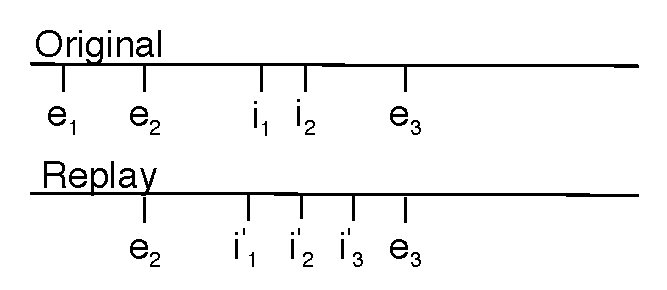
\includegraphics[width=\linewidth,height=0.8in]{../diagrams/state_machines/event_sequence.pdf}
%\end{wrapfigure}

In the general case it is always possible to construct two state machines that lead
to differing outcomes: one that only leads to the invariant violation when
we inject the next input
\emph{before} a new internal event, and another only when we inject \emph{after} a new internal
event. In other words, to be guaranteed to traverse any existing suffix that leads
to the invariant violation, we must recursively branch, trying both
possibilities for every new internal event. This implies an exponential number of
possibilities to be explored in the worst case.\footnote{
In our system~\cite{sts}, exponential search over these possibilities is not a practical option.
The heuristic our system uses when waiting for expected internal
events is to proceed normally if there are new internal events,
always injecting the next input when its last expected predecessor
either occurs or times out.}

\subsection{Modeling the Control Software}

If we assume a model of the control software's state machine, we can potentially
avoid exponential blowup. Assume we have a predicate $\Phi(\tau_P, a, b)$
that, given a prefix $\tau_P$ of events scheduled so far, and a pair of events $a$, $b$
(either external or internal), returns true whenever $\tau_P || a \rightarrow
b$ leads the software's state machine to a state $s$ s.t. some buggy state
$\hat{s}$ is reachable from $s$ along a sequence of labeled state transitions
$\alpha$, where the labels in $\alpha$
that correspond to external events are a subsequence of the remaining external inputs $E_S
\backslash \left\{ e \in \tau_P \right\}$. \colin{May want to remove the
requirement that $\alpha$ be a subsequence of external events. Alternatively,
have $\Phi$ tell us whenever injecting $a$ before $b$ would lead us {\bf off}
the original path (or an coarse-grained version of the original path)}
Here, a buggy state refers to
a state that produces a network configuration $c$ that violates a given
invariant.

For all prefixes $\tau_P || a\rightarrow b$ of $\tau_L$, if $\tau_L$ is a
superset of an MCS, then $\Phi(\tau_P, a, b)$ returns true.

For any new internal event $a$ and pending external event $b$, if
$\Phi(\tau_P, a, b)$ returns true, then we know that we can allow $a$ through
before $b$. In this way we can interleave new
internal events with our schedule of expected events $\tau_S$, and be
guaranteed to leave open the possibility of finding a divergent suffix through the
state machine that leads to an invariant violation.

\subsection{Obtaining a model}

Two ideas for obtaining $\Phi$: \\

\noindent{\bf Extrapolate from complete model.} There was a paper in
PLDI~\cite{vericon} where the authors
wrote their own controller and verified its entire state space. We could issue
queries on the state space to compute $\Phi$, and then extrapolate $\Phi$ for
other controllers assuming their state machines are sufficiently similar. \\

\noindent{\bf Infer partial models.} In general we want to
continue assuming that the control software is a black box.
Even with that constraint, we could infer a partial model of the control
software by observing its outputs across many executions, \ie~build a model
from logs. We might use Synoptic~\cite{beschastnikh2011leveraging} to compute
the model.
